\section{El último tablero}\label{terminal}

\subsection{Geometría bajo las dos leyes}

Al llegar a $K$ filas vacías y $K$ columnas vacías, el tablero residual se obtiene de sus $K^2$
cruces vacíos suprimiendo los no disponibles, que son los que comparten diagonal con una reina ya
colocada. La Figura~\ref{fig:terminal} distingue entre los cruces vacíos y la \emph{máscara}, la
matriz $A=(Y_{ij})$ de sus indicadores de disponibilidad.
\begin{figure}[htbp]
\centering
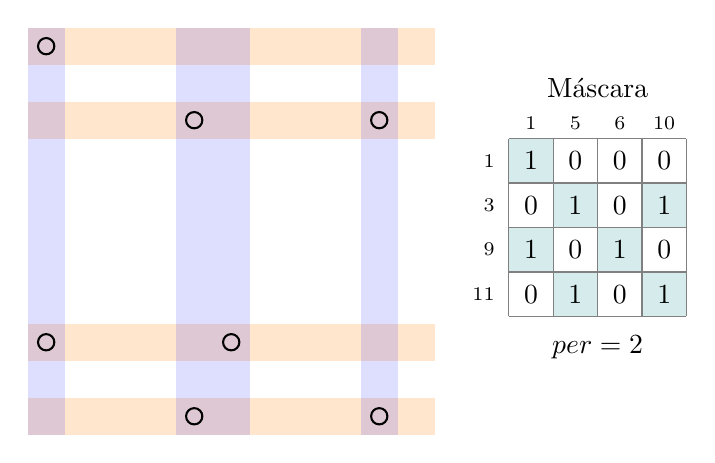
\begin{tikzpicture}[x=.47cm,y=.47cm]
 \bcuadricula{11}
 \foreach \rr in {1,3,9,11}{\fill[orange,opacity=.20] (0,{11-\rr}) rectangle (11,{12-\rr});}
 \foreach \cc in {1,5,6,10}{\fill[blue,opacity=.13] ({\cc-1},0) rectangle (\cc,11);}
 \foreach \rr/\cc in {1/1,3/5,3/10,9/1,9/6,11/5,11/10}{
  \bmarca{11}{\rr}{\cc}
  \draw[black,line width=.75pt] ({\cc-.5},{11.5-\rr}) circle[radius=.22];
 }
 \foreach \rr/\cc in {2/3,4/7,5/9,6/11,7/2,8/4,10/8}{\breina{11}{\rr}{\cc}}
 \begin{scope}[shift={(13,3.2)},scale=1.2]
  \node at (2,5.15) {Máscara};
  \foreach \indice/\original in {1/1,2/5,3/6,4/10}
   {\node[font=\scriptsize] at ({\indice-.5},4.35) {$\original$};}
  \foreach \indice/\original in {1/1,2/3,3/9,4/11}
   {\node[font=\scriptsize,anchor=east] at (-.1,{4.5-\indice}) {$\original$};}
  \foreach \rr/\cc in {1/1,2/2,2/4,3/1,3/3,4/2,4/4}
   {\fill[teal!16] ({\cc-1},{4-\rr}) rectangle (\cc,{5-\rr});}
  \draw[step=1,gray,line width=.45pt] (0,0) grid (4,4);
  \foreach \rr/\valores in {1/{1,0,0,0},2/{0,1,0,1},3/{1,0,1,0},4/{0,1,0,1}}{
   \foreach \valor [count=\cc] in \valores
    {\node at ({\cc-.5},{4.5-\rr}) {$\valor$};}
  }
  \node at (2,-.7) {$\operatorname{per}=2$};
 \end{scope}
\end{tikzpicture}
\caption{Tablero de orden once de la solución $\pi=(1,3,5,7,9,11,2,4,6,8,10)$ después de retirar las
reinas de las filas $1,3,9,11$. Las filas se numeran desde uno de arriba abajo y las columnas desde
uno de izquierda a derecha. Quedan siete reinas, dibujadas con coronas. Las bandas destacan las cuatro
filas vacías y las columnas vacías $1,5,6,10$. Los puntos rodeados señalan las casillas disponibles y
corresponden a los unos de la máscara, que conserva las etiquetas originales. La fila $1$ fuerza la
columna $1$ y entonces la fila $9$ fuerza la $6$. Las filas $3$ y $11$ pueden intercambiar $5$ y $10$,
de donde resulta el permanente $2$. Las diferencias positivas entre filas son $2,6,8,10$ y entre
columnas son $1,4,5,9$. Como los dos conjuntos son disjuntos, los cruces vacíos no comparten
diagonal.}\label{fig:terminal}
\end{figure}


Recordamos que $F$ es el suceso de permanencia de la Definición~\ref{def:regular}: la historia llega
al tamaño $K$ y todos sus tableros, incluido el de llegada $B^{(K)}$, son regulares. La figura ilustra la
geometría. En ella la fila 1 fuerza la
columna 1, por lo que toda matriz bistocástica sobre la máscara asigna masa cero a la casilla
disponible $(9,1)$. El ejemplo queda fuera de $F$. Sea
$D_K$ el suceso de que dos cruces vacíos distintos del tablero de tamaño $K$ pertenezcan a una misma
diagonal del tablero inicial. Para $m\ge 1$ escribimos
$(u)_m=u(u-1)\cdots(u-m+1)$ si
$u\ge m$, y $(u)_m=0$ si $0\le u<m$.

\begin{lema}[Diagonales compartidas en el último tablero]\label{terminal-geometria}
Bajo $\nu$ y bajo la ley $\mu$ de una solución uniforme revelada en orden uniforme independiente,
respectivamente,
\[
 \nu(F\cap D_K)\le d_{n,K}:=\frac{C K^4}{n}\,e^{C'/K},
 \qquad \mu(D_K\mid\pi)\le \frac{C K^4}{n}
\]
para toda solución $\pi$. La segunda probabilidad es respecto del orden de
revelado.
\end{lema}
\begin{proof}
En el tablero inicial hay a lo sumo $Cn^3$ pares de casillas distintas que comparten diagonal. Se
elige la primera entre $n^2$ casillas y la segunda entre a lo sumo $2(n-1)$ casillas de sus
diagonales. Para que las dos casillas de un par sean cruces vacíos en el tamaño $K$ deben quedar
vacías dos filas distintas y dos columnas distintas. En $F$ no hubo salida anterior, de modo que
\eqref{prescr} con
$s=t=2$ acota la probabilidad de cada par por $(K/n)^4e^{C'/K}$. La unión da la primera afirmación.

Para la segunda afirmación fijemos $\pi$. Las últimas $K$ filas en el orden uniforme forman un
subconjunto uniforme $I$ de tamaño $K$. Las columnas correspondientes son $\pi(I)$ y los cruces vacíos
forman $I\times\pi(I)$. La Figura~\ref{fig:testigos} muestra cómo intervienen las etiquetas de fila en
dos de esos cruces.
\begin{figure}[htbp]
\centering
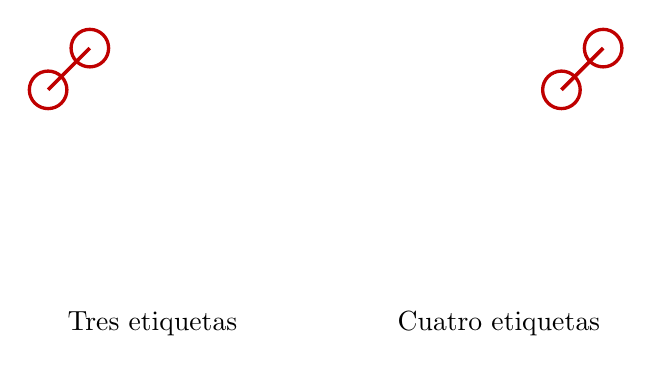
\begin{tikzpicture}[x=.53cm,y=.53cm]
 \foreach \tipo/\dx/\uno/\dos in {3/0/2/1,4/8.3/6/5}{
  \begin{scope}[shift={(\dx,0)}]
   \bcuadricula{6}
   \draw[red!75!black,line width=1.3pt] ({\uno-.5},5.5) -- ({\dos-.5},4.5);
   \bmarca{6}{1}{\uno}
   \bmarca{6}{2}{\dos}
   \draw[red!75!black,line width=1.2pt] ({\uno-.5},5.5) circle[radius=.45];
   \draw[red!75!black,line width=1.2pt] ({\dos-.5},4.5) circle[radius=.45];
   \foreach \rr/\cc in {1/2,2/4,3/6,4/1,5/3,6/5}{\breina{6}{\rr}{\cc}}
   \ifnum\tipo=3
    \node at (3,-1.1) {Tres etiquetas};
   \else
    \node at (3,-1.1) {Cuatro etiquetas};
   \fi
  \end{scope}
 }
\end{tikzpicture}
\caption{Dos testigos en el tablero de orden seis de la solución $\pi=(2,4,6,1,3,5)$. Las filas se
numeran desde uno de arriba abajo y las columnas desde uno de izquierda a derecha. Las coronas son las
reinas de $\pi$. Dos círculos unidos señalan las casillas $(i,\pi(j))$ e $(i',\pi(j'))$ que comparten
diagonal. A la izquierda, $(i,i',j,j')=(1,2,1,4)$ marca $(1,2)$ y $(2,1)$ y usa tres etiquetas
distintas. A la derecha, $(1,2,3,6)$ marca $(1,6)$ y $(2,5)$ y usa cuatro. Con sólo dos etiquetas se
tendría $\{i,i'\}=\{j,j'\}$ y $|i-i'|=|\pi(i)-\pi(i')|>0$, lo que haría que dos reinas de la solución
se atacasen.}\label{fig:testigos}
\end{figure}


Un par que comparte diagonal se escribe $(i,\pi(j)),(i',\pi(j'))$, con
\[
 |i-i'|=|\pi(j)-\pi(j')|>0,\qquad i,i',j,j'\in I.
\]
Llamamos \emph{testigo} a una cuádrupla de etiquetas $(i,i',j,j')$ que cumple esta igualdad de
distancias, pertenezcan o no a $I$. Pongamos $m=|\{i,i',j,j'\}|$. Si $m=2$, los pares de etiquetas
$\{i,i'\}$ y $\{j,j'\}$ coinciden. La
igualdad de distancias diría que las reinas de $\pi$ en las filas $i,i'$ se atacan, lo que es imposible.
Si $m=3$, fijamos $i,i'$ y cuál de las dos etiquetas se repite en cuál de las posiciones $j,j'$. La
imagen bajo $\pi$ de esa etiqueta es conocida. La otra imagen debe estar a distancia $|i-i'|$ de ella,
por lo que tiene a lo sumo dos valores posibles. Cada uno determina su etiqueta mediante $\pi^{-1}$.
Hay por tanto $O(n^2)$ testigos con tres etiquetas. Para $m=4$, fijar $i,i',j$ deja a lo sumo dos
valores para $\pi(j')$, y da $O(n^3)$ testigos.

El subconjunto $I$ contiene $m$ etiquetas fijadas con probabilidad $(K)_m/(n)_m\le(K/n)^m$ cuando
$n\ge m$. Para $n\ge4$ resulta por unión
\[
 \mu(D_K\mid\pi)\le C\left[n^2(K/n)^3+n^3(K/n)^4\right]\le CK^4/n.
\]
Bajo $\mu$, la solución y el orden se pueden completar también para historias ya detenidas. Como
$F\cap D_K\subseteq D_K$, integrar la estimación respecto de $\pi$ da también $\mu(F\cap D_K)\le
CK^4/n$.
\end{proof}
